%!TEX encoding = UTF-8

\chapter{Experimental Platform}
\label{chap:platform}

In this chapter, we provide the practical groundwork for the experiments described in the thesis.

We start by describing the iCub humanoid robot in Sec.~\ref{sec:platform:icub}.
Then, in Sec.~\ref{sec:platform:scenario} we illustrate the experimental scenario adopted in the experiments.
Finally, Sec.~\ref{sec:platform:software_architecture} presents our modular system for robot affordance learning, based on autonomous robot exploration of the world and visual processing.
The whole system will be used as a building block for the next chapters.

%%%%%%%%%%%%%%%%%%%%%%%%%%%%%%%%%%%%%%%%%%%%%%%%%%%%%%%%%%%%%%%%%%%%%%%%%%%%%%%%
\section{The iCub Humanoid Robot}
\label{sec:platform:icub}

\begin{figure}
\centering
\includegraphics[width=0.9\textwidth]{icub_green_blue_balls}
\caption[The iCub humanoid robot.]{The iCub humanoid robot (picture by Lorenzo Natale).}
\label{fig:icub}
\end{figure}

In this section, we illustrate the humanoid \emph{robot} that we will use to run the experiments of this thesis.

The robot that we use is the \emph{iCub} child-like robot~\cite{metta:2010:nn}, shown in Fig.~\ref{fig:icub}.
Its shape is similar to that of a 5-year-old child, with a height of 1~meter, a weight of~27 kilograms, and a head with fully articulated eyes~\cite{beira:2007:msc}.
The structure of the iCub is sophisticated: it has a high number of \acp{DoF}\footnote{%
At the time of writing this thesis, the iCub robot is the second humanoid robot with the highest number of \ac{DoF} (53~\ac{DoF}), being surpassed only by the ARMAR robot by Karlsruhe Institute of Technology (63~\ac{DoF}) \cite{asfour:2019:armar_family}.}% end footnote
, the majority of which are located at the arms and hands, in order to make the robot perform object grasping, dexterous manipulation as well as articulatory gestures.
The iCub also has tactile sensors and microphones: these robot sensors are not directly used in this thesis, however they are included and used in some previous studies (\cite{montesano:2008,salvi:2012:smcb}) related to this thesis.
It is an \emph{open-source platform}, having been adopted by more than~30 research groups and universities worldwide~\cite{natale:2019:icub_bookchapter}.

The open-source iCub software is, as such, the work of a large community\footnote{\url{http://www.icub.org/}, \url{https://github.com/robotology}}:~2 million \ac{LoC}, hundreds of contributors\footnote{\url{https://www.openhub.net/p/robotology}}.
Parts of the available software can be used in other applications and platforms~(i.e., without the iCub), for example the visual processing algorithms.
iCub software modules, such as the ones developed for this thesis, rely on the \ac{YARP} middleware~\cite{metta:2006:yarp,fitzpatrick:2014:yarp}.
\ac{YARP} is similar to \ac{ROS}\footnote{%
At the time of writing this thesis, \ac{ROS} \cite{quigley:2009:ros} is the \defacto{} standard middleware in robotic research.
}, % end footnote
following the same \emph{middleware} concepts about managing distributed computations across a cluster of heterogeneous computers, hardware abstractions, low-level device drivers, message passing between processes, and implementation of commonly used functionality (e.g., geometry, linear algebra, vision algorithms).

The iCub robot was developed for studying cognition and learning.
The main idea behind this platform is that it is born with simple skills, and then it can become intelligent over time by interacting with the enviroment, where the term intelligence encompasses manipulation, social skills, and interactive skills.
As a result, it can gain a certain degree of autonomy.
The usefulness of the iCub is in its completeness: it encompasses movement~(high number of motors) and the possibility to measure the external environment~(sensors), which in turn permit to study aspects of higher intelligence~(algorithms).

%%%%%%%%%%%%%%%%%%%%%%%%%%%%%%%%%%%%%%%%%%%%%%%%%%%%%%%%%%%%%%%%%%%%%%%%%%%%%%%%
\section{Experimental Scenario}
\label{sec:platform:scenario}

\begin{figure}
\centering
\includegraphics[width=0.9\textwidth]{icub_playing_with_objects_icdl-epirob2014}
\caption[The iCub robot in a playground table scenario.]{The iCub robot in a playground table scenario. Objects and tools are present in the scenario, so that the robot can interact with them, it can acquire a model of the environment derived from sensorimotor data, and it can use such a model for reasoning about the environment.}
\label{fig:icub_playing_with_objects}
\end{figure}

In our scenario, the iCub robot is positioned next to a \emph{playground table}, meaning a table which can have one or more objects on top of it.
Examples of these objects are colorful toys, sponges and elongated tools.
This scenario is designed so that the robot interacts with the objects, it acquires the model of the environment from sensorimotor data, and it can then use the acquired knowledge for reasoning about the environment.
Fig.~\ref{fig:icub_playing_with_objects} shows an example of our scenario.

In following Montesano's approach (see Sec.~\ref{sec:background:previous_works:montesano}), the variables that our model considers are related to: action, object, and effect.

Note that, when a robot interacts with its environment autonomously in a self-exploration fashion, several variables can be actively chosen by the robot, for example the motor action and the target object.
In our case, these variables are usually interventional~(see p.~\pageref{para:interventional_vars}), being set to their specific value during each experiment by the experimenter or by the robot.

\begin{figure}
\centering
\subfloat[][Grasp.]
{ \includegraphics[width=0.25\linewidth]{icub_motor_actions_grasp_lowqual} } \quad
%
\subfloat[][Tap.]
{ \includegraphics[width=0.27\linewidth]{icub_motor_actions_tap_lowqual} } \quad
%
\subfloat[][Push.]
{ \includegraphics[width=0.27\linewidth]{icub_motor_actions_push_lowqual} }
%
\caption{Examples of manipulative motor actions performed by the iCub robot onto environment objects.}
\label{fig:icub_motor_actions}
\end{figure}

Regarding the motor \emph{actions} that can be executed by the iCub during experiments, in this thesis we consider manipulative hand gestures.
These are movements performed by the \armhand{} chain of the robot, capable of touching objects in the environment from different directions.
Fig.~\ref{fig:icub_motor_actions} shows some examples of these motor actions, highlighted in white.

In this thesis, the low-level control routines to realize the motor behaviors on the iCub robot (both simulated and real) are based on works and software modules previously made available by other researchers in the iCub community~\cite{pattacini:2010:iros,roncone:2016:rss}.

Regarding the \emph{effects} in the environment that are measured using robot perception, we consider physical displacements of objects on the table, being moved by the effector of robot from the time when the robot performs the action, until a pre-defined fixed duration (number of frames) afterwards. \label{para:effects}
The effector can be the agent's bare hand or the tip of a grasped tool, as we will describe in Ch.~\ref{chap:tool}.
The physical displacement of an object is computed as the difference between the final and initial coordinates of that object on a table.
Furthermore, we consider two displacement effects: along the lateral and longitudinal direction, respectively.
By clustering the continuous sensory values, we define five discrete levels for these effects: Very Positive (VP), Low Positive (LP), No Movement (NM), Low Negative (LN) and Very Negative (VN).
These levels correspond to an object moving
\begin{itemize}
\item VP: significantly to the left (or front) from the robot's perspective;

\item LP: slightly to the left (or front);

\item NM: little or no movement;

\item LN: slightly to the right (or back);

\item VN: significantly to the right (or back).
\end{itemize}

Recall from p.~\pageref{para:BN_causality_clarification} that \acp{BN} offer the possibility of representing causal relationships, based on knowledge (specified by the experimenter arbitrarily) of the world domain being modeled.
In the experimental part of this thesis, the robot chooses an action~$A$, it executes it on an object (with certain features) $O$, and it ``causes'' the effect~$E$ as a consequence.
Since $A$ and~$O$ are given as priors, and since effects happen later in time, we attribute the meaning that $A$ and~$O$ are causes, whereas $E$ are consequences.
Still, from the point of view of \acp{BN}, $A$, $O$ and $E$ are variables with no temporal information.
In this sense, as clarified in Sec.~\ref{sec:background:theory:graphical_models}, the model does not learn causal relationships.

%%%%%%%%%%%%%%%%%%%%%%%%%%%%%%%%%%%%%%%%%%%%%%%%%%%%%%%%%%%%%%%%%%%%%%%%%%%%%%%%
\section{Software Architecture}
\label{sec:platform:software_architecture}

In this section, we introduce our software framework that permits robots to sense, learn, and use the information contained in surrounding objects as well as their affordances.
It is a modular software framework for experiments in visual robot affordances, directed at the robotics, psychophysics and neuroscience communities.
Although the system was developed for the iCub platform in particular, thanks to its modular nature, parts of the system can be used for other robots.
We make this framework publicly available\footnote{\url{https://github.com/gsaponaro/robot-affordances} \label{footnote:robot-affordances_url}}.
Below, we show how this system can be used for
(i)~the perception of relevant visual features of a robot's surrounding objects;
(ii)~reasoning about the affordances of those objects and, as a result,
(iii)~supporting the new capabilities and behaviors described in the next chapters, for example tool use and action planning.

The basic intuition behind our architecture is that a robot learns links between object shape features and their physical properties: for instance, the notion that spherical objects roll faster than cubic ones when pushed laterally with an effector~(e.g., a robot hand or a tool held in the robot's hand).

Because learning is based on a \emph{probabilistic model}, the approach is able to deal with uncertainty, redundancy and irrelevant information.
We say that affordances are learned, because we let the robot discover them from autonomous experience in its environment, and then use the learned model in various profitable ways, e.g., prediction, tool use learning, planning a sequence of actions to achieve complex goals such as stacking objects.

As mentioned in Ch.~\ref{chap:background}, Zech published a systematic taxonomy of robot affordance models~\cite{zech:2017:ab}.
According to their criteria (defined in their taxonomy),
in terms of \emph{perception} the works in this thesis classify as using an agent perspective, meso-level features, first order, stable temporality (i.e., related to static object properties that do not change over time, such as the shape of rigid objects).
In terms of \emph{development}: acquisition by exploration, prediction by inference, generalization exploitation by action selection and language, and offline learning.

\subsection{Visual Pipeline}
\label{sec:platform:software_architecture:visual_pipeline}

\begin{figure}
    % align option is for linebreaks, https://tex.stackexchange.com/a/124114
    % RGB color is light gray
    \tikzstyle{block} = [rectangle, draw, thick, align=left, fill={rgb,255: red,234; green,236; blue,239}]
    %
    \centering
    \resizebox{0.9\textwidth}{!}{ % https://tex.stackexchange.com/a/363884
    \begin{tikzpicture}
    \node (robot_cam) [draw=none, circle, minimum size = 1mm, align=left] at (0, 0) {robot \\ camera};
    \node[draw=none, label={\tiny color image}, text width=1.25cm] (inv1) [right=of robot_cam, xshift=-0.75cm] {};
    \node[block, right=of inv1, xshift=-0.75cm] (segm) {segmentation};
    \node[draw=none, label={\tiny binary image}] (inv2) [right=of segm] {};
    \node[block, right=of inv2] (bd) {Blob \\ Descriptor};
    \node[block, below=of inv2] (sl) {Sequential \\ Labeler};
        \node[block, right=of bd] (bn) {Bayesian \\ Network \\ affordance \\ knowledge};
    %
    \draw[affarrow] (robot_cam) -- (segm.west);
    \draw[affarrow] (inv2.center) -- (sl.north);
    \draw[affarrow] (segm) -- (bd);
    \draw[affarrow] (sl) -| node[above, text width=1.25cm, xshift=-0.4cm]{\tiny labeled image} (bd);
    \draw[affarrow] (bd) -- node[above, text width=1.25cm, xshift=0.1cm, yshift=0.5cm]{\tiny shape features} (bn);
    \draw[->, dotted] (inv1.center) |- ([shift={(0mm,-26mm)}]inv1.center) -- node[below]{\tiny (optional connection, for visualization purposes)} ([shift={(0mm,-20mm)}]bd.south) -| ([shift={(5mm,0mm)}]bd.south);
    %
    \draw ([shift={(3mm,14mm)}]segm.north east) to[out=-90,in=0,distance=3.5cm] ([shift={(-5mm,-20mm)}]inv1.south);
    \node[text width=3.4cm, align=right] at (3.5, 1.4) {\small \emph{existing work by other researchers} \tiny (see p.~\pageref{para:lbpExtract})};
    \node at (7.3, 1.4) {\small \emph{our contributions}};
    \end{tikzpicture}
    } % end resizebox
    \caption[Our pipeline for computing visual affordance features.]{Our pipeline for computing visual affordance features. Boxes indicate software modules, arrows indicate data flow connections, dotted arrows indicate optional data flow connections.
    See text for details, and Fig.~\ref{fig:shape_features_pipeline} for an example computation.}
    \label{fig:our_aff_pipeline}
\end{figure}

\begin{figure}
\centering
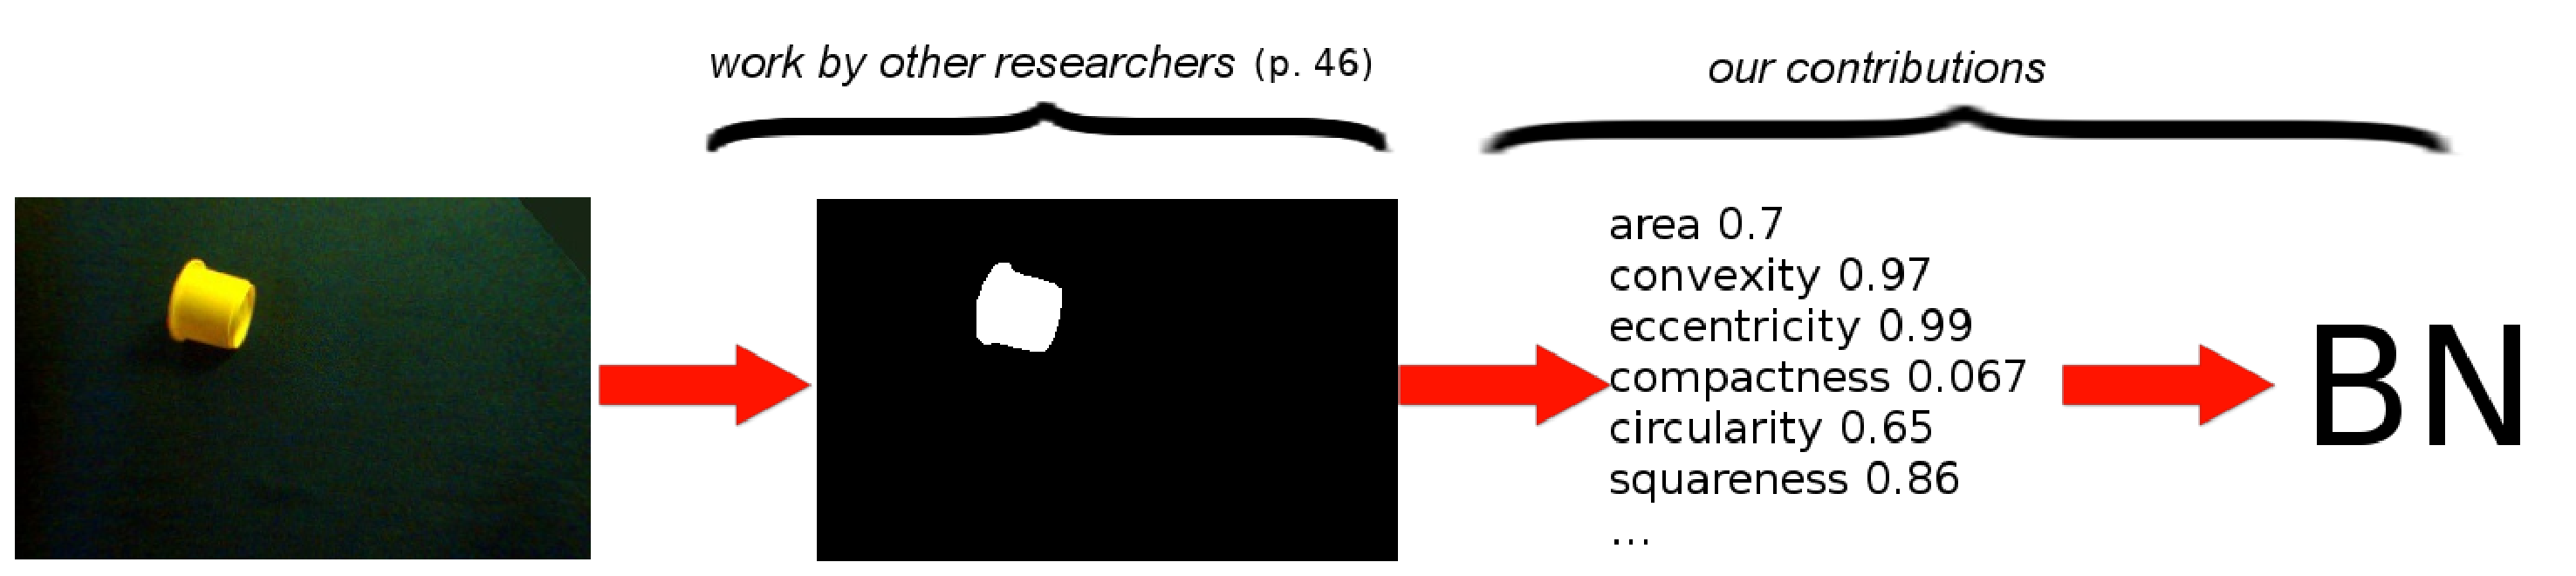
\includegraphics[width=0.9\textwidth]{shape_features_pipeline3_link_to_p46}
\caption[Example computation of extracting salient shape features for affordances.]{Example computation of extracting salient shape features for affordances.
From left to right: robot camera color image, binary segmentation image, shape features, \acl{BN} affordance knowledge.
The set of extracted shape features characterizes the object.
This set is then used to train the robot affordance knowledge model, and to perform inference queries on an affordance database.
See also Fig.~\ref{fig:our_aff_pipeline} for the diagram of software modules.}
\label{fig:shape_features_pipeline}
\end{figure}

The objective of this section is to illustrate a real-time~(30 fps), versatile and easy-to-use visual processing software that can be used in different scenarios such as robot perception, higher-level cognitive reasoning~(e.g., reasoning about the possibilities afforded by perceived objects) and related studies.

Starting from the beginning of such a perception and reasoning pipeline, let us first focus on visual features.
Computing features of interest of objects present in images is a frequent task in cognitive robotics.
For example, for the iCub humanoid robot this fundamental capacity was required during the research projects RobotCub\footnote{\url{http://www.robotcub.org/}} and POETICON++\footref{footnote:poeticon++}, where the robot had to see, characterize and grasp objects located on a playground table scenario, as described in Sec.~\ref{sec:platform:scenario}.
The exact requirements and subtleties vary slightly among different projects, setups and demonstrations.

Recall from Sec.~\ref{sec:motivation:neuro:twostreams} that the two-streams hypothesis of neuroscience speculates that visual perception occurs across two separate pathways: ventral and dorsal.
The former is mainly related to object recognition and categorization, the latter guides object-directed actions~(e.g., reaching and grasping).
We now illustrate the main components of our robot affordance pipeline, which is inspired by the dorsal pathway, in the sense that it does not require to know or recognize the category of objects, instead it reasons on their low-level shape features, and it permits the agent to act fast.

Fig.~\ref{fig:our_aff_pipeline} shows the organization of our pipeline, where boxes indicate conceptual~(and software) modules, arrows indicate data flow connections, and dotted arrows indicate optional data flow connections.
Fig.~\ref{fig:shape_features_pipeline} shows an example computation.
At the end of the pipeline, shape features are computed.
They serve as the data (about world objects) for the \ac{BN} computational implementation of the affordance knowledge.
In particular, using clustering of the continuous sensory values, we define three discrete levels for each shape feature: Low~(L), Medium~(M), and High~(H). \label{para:objects}

\begin{table}
\caption{Shape descriptors.}
\label{tab:descriptors}
\centering
\begin{tabular}{lp{0.6\columnwidth}}
\toprule
descriptor & definition \\
\midrule
area & number of blob pixels, normalized w.r.t. a constant \\
convexity & ratio between convex hull perimeter and object perimeter \\
eccentricity & ratio between minor and major axes of best-fit ellipse \\
compactness & ratio between object area and squared external contour perimeter \\
circularity & ratio between object area and area of minimum-enclosing circle \\
squareness & ratio between object area and area of minimum-enclosing rectangle \\
convexity defects & number of ``holes'' along blob contour \\
image moments & weighted averages of the blob pixels' intensities \\
\bottomrule
\end{tabular}
\end{table}

The modules are the following:
\begin{description}
    \item[segmentation] A visual module that takes as input a color image obtained from a robot camera, and outputs a binary image containing white pixels on the location of the objects, black pixels elsewhere~(i.e., background).
    Because the overall architecture is modular, it is possible to plug and play different segmentation implementations and algorithms as this module, provided that they have the required input and output format.
    The implementation that we adopt for the experiments in this thesis~(written by other researchers\footnote{%
        \texttt{lbpExtract} software module, written by Vadim Tikhanoff and available at \url{https://github.com/robotology/segmentation}
    }) % end footnote
    uses \acp{LBP}~\cite{ojala:2002:pami} for analyzing the texture of objects on a table in front of the robot, based on comparing the intensity of each pixel with its neighbors and representing this relationship with a histogram of binary numbers. \label{para:lbpExtract}

    \item[Sequential Labeler] A visual module that takes as input a binary segmentation image, and extracts as output the connected components contained therein (i.e., contiguous subsets of pixels). We call the output image \emph{labeled}, meaning that its pixels correspond to identifiers of the segmented objects: pixels are set to zeros over the background, to ones over the first segmented object, to twos over the second segmented object, etc.

    \item[Blob Descriptor] A visual module that, from the binary and labeled images, computes a vector of descriptors for each segmented object present in the scene.
    This module performs measurements on the connected components~(obtained by the two modules above), in order to extract some of their salient characteristics.
    The features that we extract are pre-categorical shape descriptors~\cite{zhang:2004:shape} computed as geometric relationships between perimeter, area, convex hull and approximated shapes of the segmented silhouettes of the objects in front of the robot.
    We list these shape descriptors in Table~\ref{tab:descriptors}.
\end{description}

The different types of images being processed and passed along between the modules are:
\begin{description}
    \item[color image] as acquired from the robot camera driver;

    \item[binary segmentation image,] which separates the objects of interest from the background. This image thus contains the contours of the object shapes, which we call \emph{blobs};

    \item[labeled image,] containing the uniquely-numbered connected components corresponding to the visual blobs: the pixels of the~$i^{\text{th}}$ blob are numbered~$i$, the background pixels are numbered zero.
\end{description}

\subsection{Impact}
\label{sec:platform:software_architecture:impact}

In addition to being applied for this thesis and other works authored by \myFullName, our visual affordances system has also been used by external researchers outside our scope,
namely:
\begin{itemize}
    \item in a developmental psychology work that links the visual appearance of objects with language learning on an iCub robot~\cite{morse:2016:cogsci}, and

    \item in studies about robot tool affordances which rely on the \emph{deep learning} paradigm instead of \aclp{BN}~\cite{dehban:2016:eccvws,dehban:2016:icra,dehban:2017:humanoids}.
\end{itemize}
